\subsection{Terminologie \cite{MOP}}

\begin{description}
  \item[Individu]: Une solution au probl\`eme pos\'e; elle peut \^etre plus ou moins performante.
  \item[Population]: Ensemble des individus trait\'es simultan\'ement par l'algorithme \'evolutionnaire.
  \item[G\'en\'erations]: It\'erations durant lesquelles \'evolue la population, jusqu'\`a ce qu'un crit\`ere d'arr\^et soit v\'erifi\'e.
  \item[Parent]: Individu soumis \`a un op\'erateur.
  \item[Enfant]: Individus r\'esultant de l'application d'un op\'erateur.
\end{description}


\subsection{Principe}
Le principe d'un algorithme g\'en\'etique est d'appliquer une variation (mutation et/ou croisement) sur un ou plusieurs individus. Dans le cas d'une mutation, un individu est modifi\'e al\'eatoirement, la taille de la population n'est donc pas modifi\'ee. Un croisement s'applique sur n individus de la population. Il s'agit de combiner suivant certains crit\`eres ces individus.\\
Pour pouvoir appliquer une variation, il est n\'ecessaire de d\'efinir un codage qui repr\'esentera n'importe quel individu d'une population. Cela permet de r\'ealiser des coupures ou des \'echanges par exemple sur les individus.\\

La qualit\'e d'un individu peut d\'eterminer son taux d'utilisation pour la reproduction. Pour la d\'eterminer, il faut d\'efinir une fonction de performance (\textit{fitness function}) affectant \`a chaque individu une valeur de performance. L'inconv\'enient d'une telle fonction est qu'il faut la recalculer \`a chaque it\'eration pour mettre \`a jour la population.
Plusieurs strat\'egies de s\'elections peuvent \^etre utilis\'ees: 
\begin{itemize}
  \item[-] la s\'election d\'eterministe : seuls les n meilleurs individus sont s\'electionn\'es,
  \item[-] les tournois stochastiques : les n meilleurs individus sont choisis chacun avec une probabilit\'e comprise entre 0,5 et 1.
  \item[-] les tournois d\'eterministes : la s\'election est al\'eatoire.
  \item[-] le remplacement de g\'en\'eration : on ne garde que les enfants
\end{itemize}

\begin{figure}
  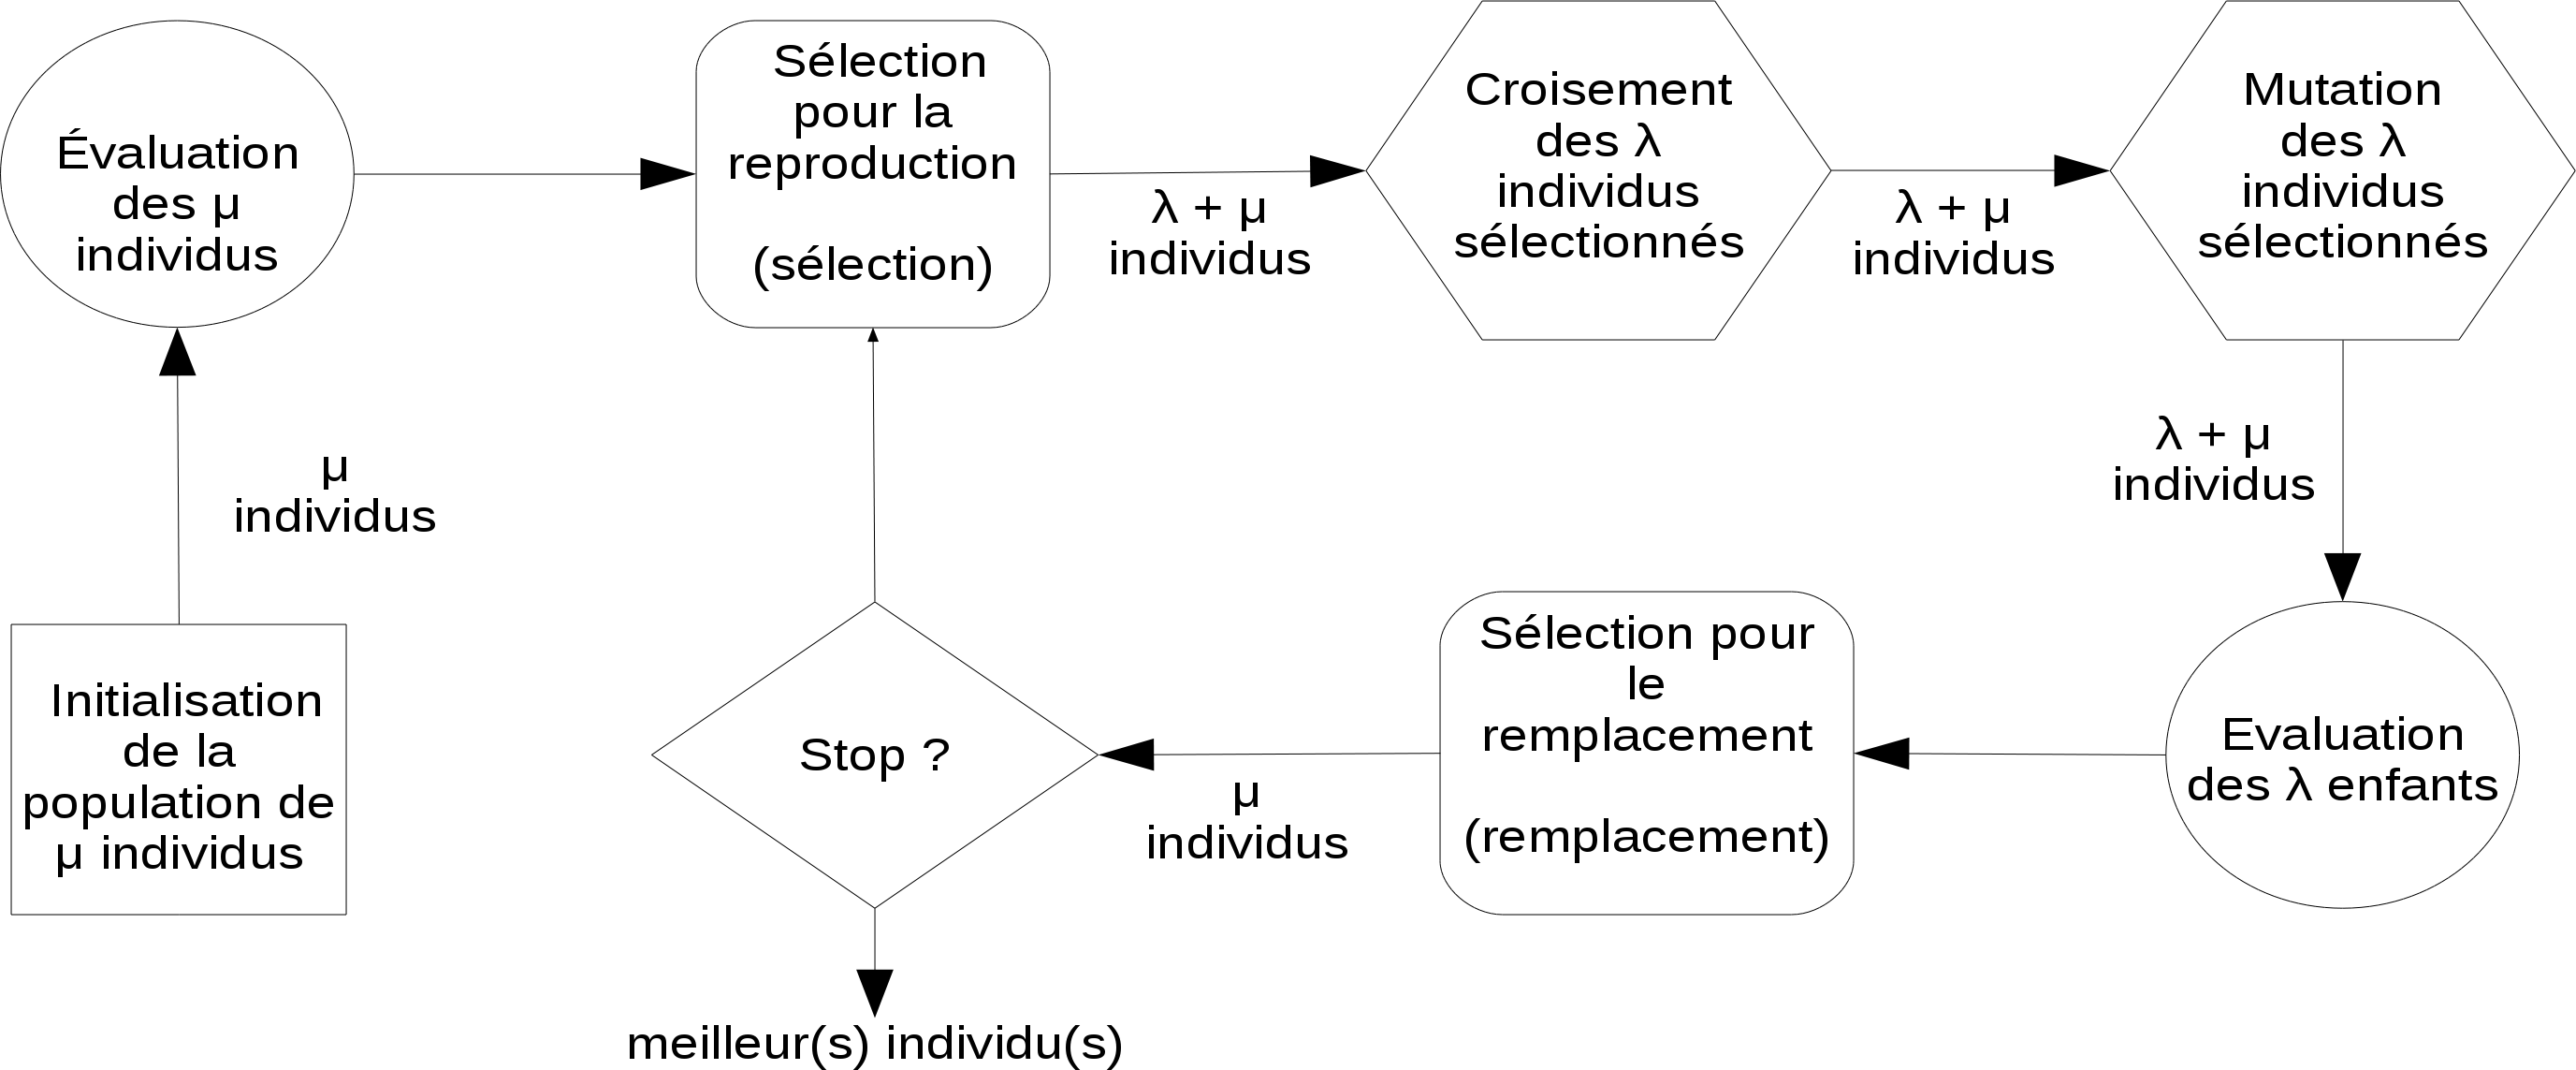
\includegraphics[width=\linewidth]{img/cycle.png}
  \caption{L'algorithme \'evolutionnaire g\'en\'erique \cite{MOP}}
\end{figure}

Le probl\`eme ``Ricochet Robots'' peut \^etre mod\'elis\'e par une matrice d'adjacences. Un individu sera rep\'esent\'e par un vecteur contenant une liste de sommets adjacents. Apr\`es avoir construit la population, un individu est choisit au hasard, et supprim\'e des autres listes afin de ne pas faire demi tour. Cet individu est ensuite crois\'e avec un autre selon une strat\'egie \`a d\'efinir. On recommence ce processus tant qu'un chemin valide n'a pas \'et\'e trouv\'e (chemin du robot \`a sa cible).\\
Il est \`a noter que dans ce probl\`eme, plusieurs populations sont envisageables (une par robot). Il faut donc d\'efinir les interactions entre celles-ci. De plus, il faut d\'efinir une ``fitness function''. Ici, elle devra prendre en compte la taille du vecteur (le nombre de coups effectu\'es), et le fait que la cible appartient ou non \`a la liste.
